%
% File acl2021.tex
%
%% Based on the style files for EMNLP 2020, which were
%% Based on the style files for ACL 2020, which were
%% Based on the style files for ACL 2018, NAACL 2018/19, which were
%% Based on the style files for ACL-2015, with some improvements
%%  taken from the NAACL-2016 style
%% Based on the style files for ACL-2014, which were, in turn,
%% based on ACL-2013, ACL-2012, ACL-2011, ACL-2010, ACL-IJCNLP-2009,
%% EACL-2009, IJCNLP-2008...
%% Based on the style files for EACL 2006 by 
%%e.agirre@ehu.es or Sergi.Balari@uab.es
%% and that of ACL 08 by Joakim Nivre and Noah Smith

\documentclass[11pt,a4paper]{article}
\usepackage[hyperref]{acl2021}
\usepackage{times}
\usepackage{latexsym}
\usepackage{graphicx}
\usepackage{mathtools}
\renewcommand{\UrlFont}{\ttfamily\small}

% This is not strictly necessary, and may be commented out,
% but it will improve the layout of the manuscript,
% and will typically save some space.
\usepackage{microtype}

%\aclfinalcopy % Uncomment this line for the final submission
%\def\aclpaperid{***} %  Enter the acl Paper ID here

%\setlength\titlebox{5cm}
% You can expand the titlebox if you need extra space
% to show all the authors. Please do not make the titlebox
% smaller than 5cm (the original size); we will check this
% in the camera-ready version and ask you to change it back.

\newcommand\BibTeX{B\textsc{ib}\TeX}

\title{EN.601.769 Assignment 2: Synthesis Paper}

\author{First Author \\
  Affiliation / Address line 1 \\
  Affiliation / Address line 2 \\
  Affiliation / Address line 3 \\
  \texttt{email@domain} \\\And
  Second Author \\
  Affiliation / Address line 1 \\
  Affiliation / Address line 2 \\
  Affiliation / Address line 3 \\
  \texttt{email@domain} \\}

\date{}

\begin{document}
\maketitle
%\begin{abstract}
%Shpeks
%\end{abstract}

\section{A\&R Factors}\label{sec:ar-factors}

\newcite{abend-rappoport-2017-state} described a plethora of factors to classify existing Semantic Representations of Text (SRTs). The described factors include: \textbf{connection to lexical items} (can SRTs be mapped to the original text?) and \textbf{syntax} (is there correspondence between syntactic and semantic representations?), \textbf{cross-sentence annotations} (do SRTs support cross-sentence relations and larger discourse contexts?), \textbf{logical structure} (for symbolic SRTs, what is the underlying formal language?), \textbf{inference capabilities} (how well suited the SRTs are for downstream inference tasks, say recognizing textual entailment?), \textbf{universality} (how well does each semantic scheme generalizes across languages?) and \textbf{annotation effort} (is the annotation fully manual? do we need skilled experts or crowd workers? how long does the annotation take?).

\section{Proposed Factors}\label{sec:proposed-factors}
\subsection{Options Considered}

To suggest two new factors, I took a practical standpoint, considering what a potential end-user, interested in extracting events from text, needs to be aware of, before locking in their application or model with a particular SRT. The options I considered were: \textbf{representations of event predicates} (what is the vocabulary of event predicates?), \textbf{initial layer of annotation} (are annotations done over raw texts? or dependency trees? or another existing SRT?), \textbf{completeness of annotations} (is the goal to annotate eveyrthing in a given corpus? or provided a certain number of ``exemplars'' per each label, akin to \cite{baker-etal-1998-berkeley-framenet}?), \textbf{mappings to other well-known resources} (can we map from a given SRT to, say, FrameNet? PropBank? VerbNet?) and \textbf{corpus domain} (what domain(s) does the gold annotated data come from?).

\subsection{Final Choice of Factors}
I chose \textbf{representations of event predicates} and \textbf{corpus domain} as my two factors.

%\textbf{Initial layer of annotation} indicates what information needs to be readily available (or which Information Extraction toolkits need to be run) in order to produce new gold (or silver) annotated data given an SRT. It also indirectly provides a lower bound of the running time for the IE component, which might be crucial for large-scale applications. As an example, if a hypothetical SRT $A$ is annotated over FrameNet, then the amount of gold data for SRT $A$ is theoretically limited by the amount of gold FrameNet data, and the IE toolkit producing silver $A$-annotated text requires first running the FrameNet IE toolkit (incurring all runtime and error propagation costs associated with it).

\textbf{Representations of event predicates} specify what counts as an event predicate and how is it represented. Is it a lexical unit with an associated verb sense, as in PropBank, or a separate label that generalizes multiple lexical units, as in VerbNet and FrameNet? I chose this particular factor for a practical reason: for my final project, I am interested in Causal Discovery over arbitrary frequent event sets. The existing CD tools expect reasonably sized vocabularies of events, and minimally the size of the event vocabulary is at least as big as the size of the event predicate vocabulary $|V_{Pred}|$. While for all the representations considered in this report this number is on the order of all unique English verbs ($|V_{Pred}| \sim 10^4$), there exist more parsimonious representations such as FrameNet ($|V_{Pred}| = 1221$) and VerbNet ($|V_{Pred}| \sim 10^2$).

\textbf{Corpus domain}, broadly, specifies the sampling distribution of all the existing gold annotated data\footnote{However, for the purposes of this report, I will only consider the corpora mentioned in the respective papers, where each SRT was introduced.} for a given SRT. More specifically, it controls the genre and the style of texts, the distribution of tokens (which tokens are considered frequent? rare?) and various document-level statistics (what's the average length of a passage? a document?). Why and where is the corpus domain important? 
% TODO: rewrite
Indeed, all the schemes considered here claim to be capable of providing general-purpose representations. However, the end-user still needs to be aware if, say, their downstream task is inference in the domain of science fiction literature, and all the gold annotated data for an SRT of choice is newswire texts or Reddit posts.

\subsection{Classification of Schemes}
\paragraph*{AMR}
To represent events (or concepts in the paper's terminology), AMR \cite{banarescu-etal-2013-abstract} uses \textbf{PropBank} \cite{kingsbury-palmer-2002-treebank,palmer-etal-2005-proposition} \textbf{framesets}. A single concept might be realized into different lexical forms. For instance, the concept ``desire-01'' might be realized as a verb (``desire''), a noun (also ``desire''), or an adjective (``desirous''). The concepts need not necessarily be verbal: some adjectives are mapped into verbal predicates (e.g. ``be aware (of X)'' $\rightarrow$ ``realize-01'') while for others the adjectives themselves are used as predicate names (e.g. ``be-efficient (at X)'' $\rightarrow$ ``efficient-01''). The AMR bank is constructed manually over exemplar sentences from domains such as \textbf{tutorials, newswire, web data, novels}, and \textbf{broadcast conversations}.

\paragraph*{UCCA}
The equivalent of an event in UCCA \cite{abend-rappoport-2013-universal} is called a \textit{scene}. Each  scene (further subcategorized as a Process or a State) is represented as a DAG where nodes are lexical units and edges are categories (e.g. Process, State, Participant, Adverbial). Therefore, event predicates are simply \textbf{English words} in UCCA. Predicate arguments are not further sub-typed beyond the Participant category. The annotated corpus is mostly  based on \textbf{English Wikipedia articles about celebrities}. This domain is chosen for its diversity and accessibility to annotators.

\paragraph*{GMB} Semantic representations of GMB \cite{basile-etal-2012-developing} are based on Boxer \cite{bos-2008-wide} which represents events as neo-Davidsonian-style predicates, where event predicates are simply \textbf{English words} and event arguments are expressed with an inventory of VerbNet \cite{kipper2008large} thematic roles. GMB is annotated over open-domain text corpora such as \textbf{newswire} (from Voice of America), \textbf{country descriptions} (from the CIA Factbook), \textbf{a collection of texts from Open American National Corpus}, and \textbf{Aesop's fables}.

\paragraph*{UDS} Predicate extraction in UDS \cite{white-etal-2016-universal} is handled via PredPatt. \textbf{PredPatt predicates} are built recursively from a Universal Dependency parse via 1) predicate root identification, where certain tokens such as governors of \textit{nsubj/dobj}, or dependendents of \textit{acl/ccomp} are designated as predicate roots, 2) predicate phrase extraction, where the subtree of a root token is expanded until a stop critetion is met. As an example, a PredPatt predicate could be simply a verb (``finds'') or a verb with a negation and an adverbial modifier (``did not sleep quietly''). The paper had preliminary annotations over exemplar sentences from PropBank and SemLink. A larger UDS1.0 dataset,  collected later by \newcite{white2019universal}, provides an annotation layer over English Web Treebank \cite{bies2012english} and covers \textbf{weblogs, newsgroups, email, reviews}, and \textbf{QA} genres.


\section{QA-SRL}
Here, I will discuss QA-SRL \cite{he-etal-2015-question} through the lens of the A\&R factors (Section \ref{sec:ar-factors}) and the factors proposed in the report (Section \ref{sec:proposed-factors}).

\subsection{Existing Factors}
QA-SRL deals with \textit{argument annotation}: given a sentence $s$ and a pre-identified verbal predicate $v$, the annotators must produce a set of wh-questions that contain $v$ and whose answers are phrases in $s$. Possible predicates are chosen to be verbs from $s$. Answer spans are effectively subsequences of the words from $s$ and need not be contiguous. As such, they are \textbf{connected lexically} (but \textbf{not syntactically}) to a sentence $s$ (and its syntactic representation). The annotations are done \textbf{on a sentence level} and \textbf{no explicit logical structure is assumed}. The \textbf{inference capabilities} of QA-SRL are also \textbf{limited} since QA-SRL deals with identifying arguments of an existing event, and not the whole event. Both question generation and answer identification experiments are performed in English, but the proposed QA-driven approach could be easily extended to other languages and is thus \textbf{universal}. Finally, the annotation took \textbf{6-9 minutes per sentence}, depending on the domain of the text. The annotators were \textbf{crowd workers}. Screening and training them took less than 2 hours on average.

\subsection{Proposed Factors}
The corpus domains covered in QA-SRL experiments are \textbf{newswire} texts (subsampled from the training data of CoNLL-2009 shared task) and \textbf{Wikipedia}. The data comes in the form of 3000 exemplar sentences with nearly 8000 verbs. Since the goal of QA-SRL is to identify arguments, the predicates have been pre-identified as simply \textbf{all the English verbs from the exemplar sentences}\footnote{The annotators had the ability to discard the irrelevant verb predicates; around 2-3\% of predicates were discarded.} using either gold or predicted POS tags, depending on the corpus domain. 

\section{Story Generation with Semantic Plans}
\begin{figure}[t!]
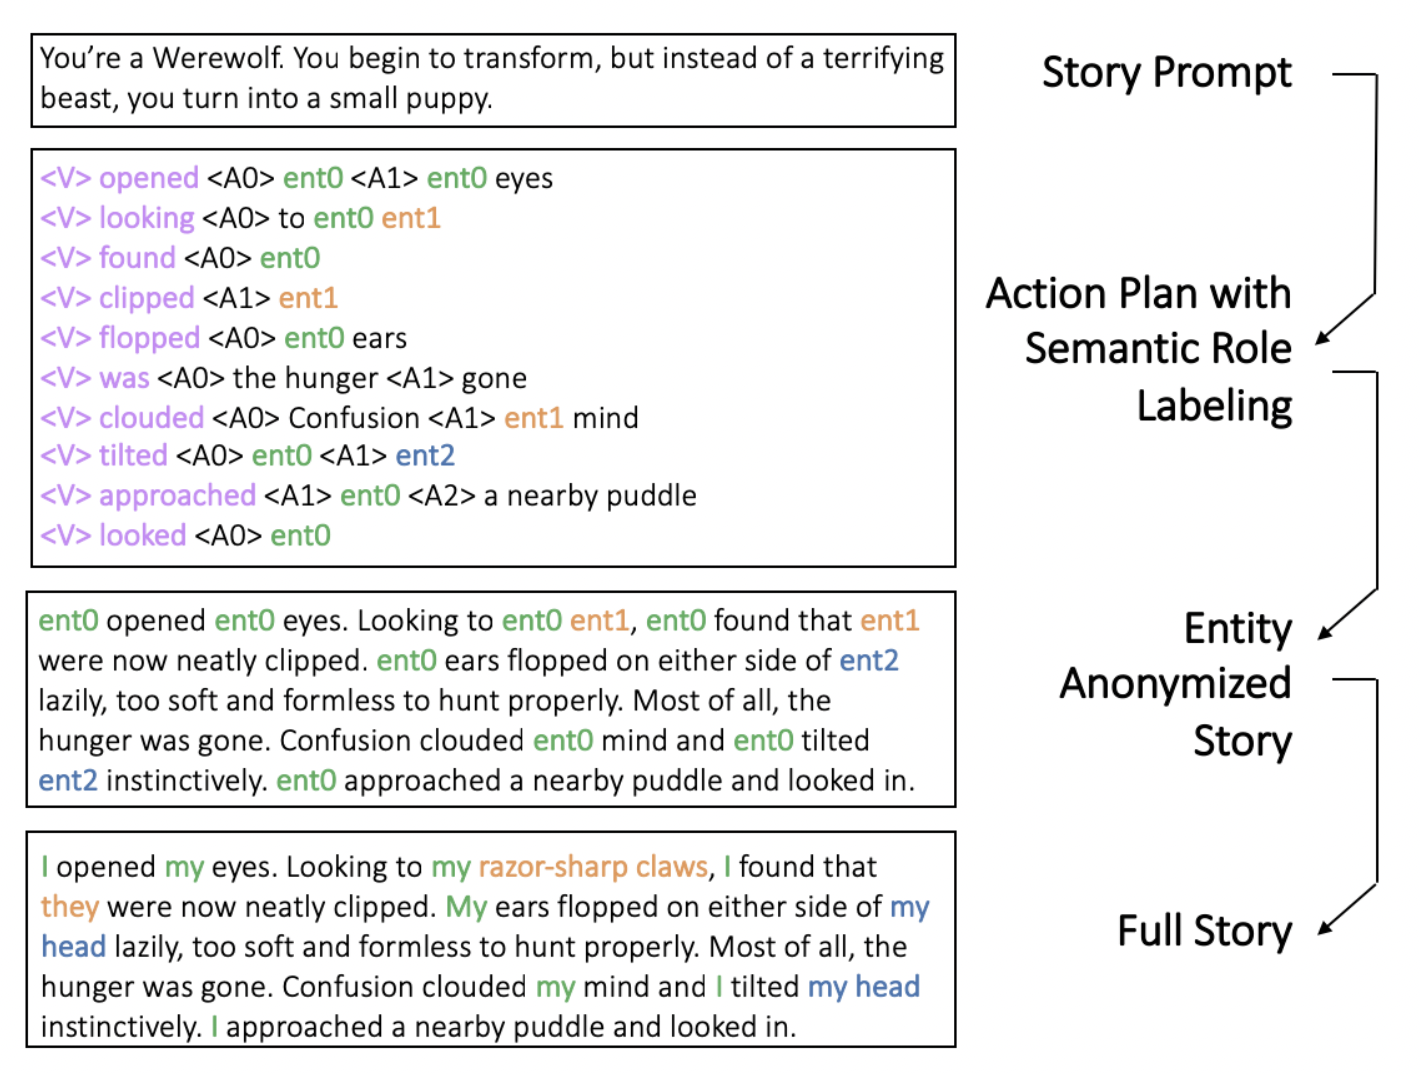
\includegraphics[width=0.5\textwidth]{fan19_storygen.png}
\caption{Story generation pipeline of \newcite{fan2019strategies}. PropBank framesets and roles are used in Action Plans.}\label{fig:fan19}
\end{figure}

\subsection{Introduction}
The task of Story Generation is often decomposed into a planning and a realization stage \cite{yao2019plan,fan2019strategies,rashkin2020plotmachines}. In the first stage, given a short prompt, a plan (also called an outline, or a skeleton) is generated. In the second stage, a model (typically, a conditional language model) realizes the plan into a coherent natural language story. This decomposition allows for more explainable generation and facilitates interactive writing \cite{goldfarb2019plan}.

Existing work on story planning demonstrates a variety of representations. \newcite{chen2019learning} use external summarization models.  \newcite{yao2019plan} extract most important words of each story sentence based of word frequency. \newcite{fan2019strategies} identify PropBank predicates and their arguments with external pretrained models. They then employ coreference resolution to identify mention chains across the extracted predicates and rename (``anonymize'') those to \texttt{ent0}, \texttt{ent1}, $\ldots$ to make story plans more general. An example of their PropBank-based story plan and a realized story is shown on \autoref{fig:fan19}.

In this section, I argue for a more semantically rich story plan representation based on \textbf{FrameNet} frames as well as \textbf{WikiData} entities (qnodes) and relations (pnodes). This proposed representation is similar to \newcite{ou2021infillmore} but elaborates more on the representation of arguments and relations.

\subsection{Predicate Representation}
To represent events succinctly while generalizing over multiple lexical forms, I propose using FrameNet frames as event predicates. As shown by  \cite{ou2021infillmore}, such a representation for story plans is able to give enough guidance for the realization model while not constraining the generation too much. It is also more \textbf{universal} than the language-specific VerbNet, GMB, and UCCA and can potentially improve the \textbf{sampling complexity} of a PropBank-based planning model of \newcite{fan2019strategies}, owing to smaller event predicate vocabulary and fewer parameters to learn as a result.

Practically, when mining plans from stories, it might be reasonable to keep the most salient frames only, similar to how \newcite{yao2019plan} only keeps one keyword per sentence. To that end, PredPatt can be used to first identify spans that represent event predicates, and then frame extraction may be constrained to these spans only. Alternatively, one can identify the most event salient spans \cite{liu2018automatic} and similarly constrain frame extraction to event salient spans only.

\subsection{Argument Representation}
The anonymization process of \newcite{fan2019strategies} is reasonable but discards all the typological information about entities. After anonymization, it is unclear from the plan whether an entity was a human, an animal, a commodity, or a location. I propose storing entity types as part of the story plan. Entity types may be obtained by linking the entities to WikiData, and traversing the ``subclass of'' relation until a desired entity typing level is reached. Using this approach, e.g. ``poodle'' (Q38904) can be typed as ``dog'' (Q144) $\rightarrow$ ``pet'' (Q39201) $\rightarrow$ ``domesticated animal'' (Q622852)'' $\rightarrow$ ``animal'' (Q729).

\subsection{Representing Entity Relations}
Suppose we want the entities in a story to be related in a particular way. For example, we may want to say that \texttt{ent0} is a person who is employed at the \texttt{ent1} university. Or say that \texttt{ent0} is a person who is employed at a particular university, say Q193727\footnote{\url{https://www.wikidata.org/wiki/Q193727}}. This information might be generated automatically by the planning model, or provided manually by a human. Similar as before, we can employ WikiData and represent such a relation as a typed edge: \texttt{ent0} $\xrightarrow[\text{P108}]{}$ \texttt{ent1}, where P108 is a WikiData property representing employment.


\bibliographystyle{acl_natbib}
\bibliography{anthology,hw2}

%\appendix


\end{document}
